\documentclass[tikz]{standalone}

\usepackage{pgfplots}
\pgfplotsset{compat=newest}

\begin{document}
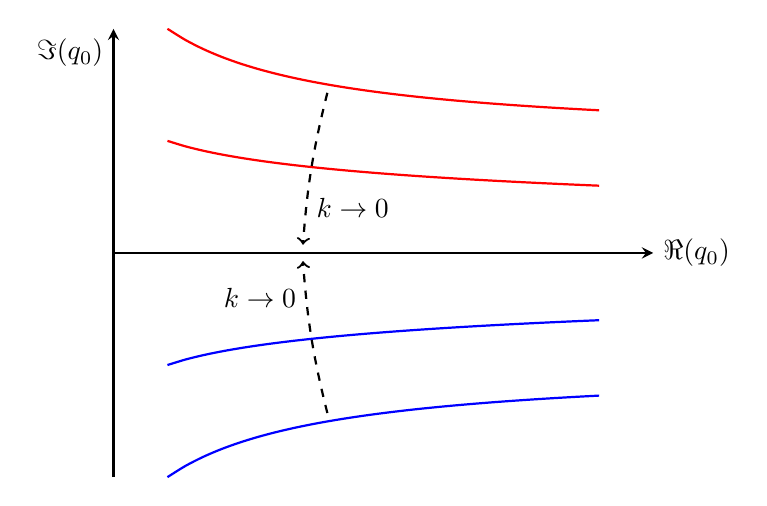
\begin{tikzpicture}
  \begin{axis}[
      xmin=0,xmax=10,
      xlabel = $\Re(q_0)$,
      ylabel = $\Im(q_0)$,
      smooth,axis lines=middle,thick,
      every tick/.style = {thick},
      xlabel style = right,
      ylabel style = below left,
      ticks=none]

    \addplot[color=red,domain = 1:9]{1/(sqrt(x)+2)};
    \addplot[color=red,domain = 1:9]{1/(x+2) + 1/3};

    \addplot[color=blue,domain = 1:9]{-1/(sqrt(x)+2)};
    \addplot[color=blue,domain = 1:9]{-1/(x+2) - 1/3};

    \draw[dashed,shorten >=3,shorten <=3] (4,0.5) edge [->,bend right=5] node[near end,right] {$k \to 0$} (3.5,0);
    \draw[dashed,shorten >=3,shorten <=3] (4,-0.5) edge [->,bend left=5] node[near end,left] {$k \to 0$} (3.5,0);

  \end{axis}
\end{tikzpicture}
\end{document}
